\documentclass[11pt,a4paper]{article}
\usepackage[margin=1in]{geometry}
\usepackage{amsmath,amssymb}
\usepackage{graphicx}
\usepackage{hyperref}
\usepackage{listings}
\usepackage{xcolor}
\usepackage{algorithm}
\usepackage{algpseudocode}
\usepackage[margin=1in]{geometry}
\usepackage{amsmath,amssymb}
\usepackage{graphicx}
\usepackage{xcolor}
\usepackage{tikz}
\usetikzlibrary{matrix,decorations.pathreplacing,positioning, calc}

% Code listing style
\lstset{
    language=Python,
    basicstyle=\ttfamily\small,
    keywordstyle=\color{blue},
    commentstyle=\color{green!60!black},
    stringstyle=\color{red},
    showstringspaces=false,
    breaklines=true,
    frame=single,
    numbers=left,
    numberstyle=\tiny\color{gray}
}

\title{\textbf{Rayleigh Wave Forward Modeling in Layered Elastic Media}\\
\large Implementation Notes and Results}
\author{Anurag Mishra}
\date{\today}

\begin{document}

\maketitle

\begin{abstract}
This document presents a comprehensive implementation of Rayleigh wave forward modeling in layered isotropic elastic media using the Thomson-Haskell propagator matrix method. The implementation includes dispersion curve computation, eigenfunction analysis, and apparent phase velocity calculation. Results are validated against theoretical expectations for multiple test cases.
\end{abstract}

\tableofcontents
\newpage

\section{Introduction}

\subsection{Problem Statement}
Rayleigh waves are surface waves that propagate along the free surface of an elastic medium. In layered media, these waves exhibit \textbf{dispersion}: their phase velocity depends on frequency. Understanding this dispersion is crucial for:
\begin{itemize}
    \item Near-surface seismic imaging
    \item Geotechnical site characterization
    \item Non-destructive testing
    \item Seismic hazard assessment
\end{itemize}

\subsection{Objectives}
\begin{enumerate}
    \item Implement forward modeling to compute Rayleigh wave dispersion curves
    \item Calculate mode shapes (eigenfunctions) showing wave energy distribution with depth
    \item Compute apparent phase velocity representing observable multimodal interference
    \item Validate implementation against physical expectations
\end{enumerate}

\section{Theoretical Framework}

\subsection{Governing Equations}

For an isotropic elastic medium, the equation of motion is:
\begin{equation}
\rho \ddot{\mathbf{u}} = (\lambda + \mu) \nabla(\nabla \cdot \mathbf{u}) + \mu \nabla^2 \mathbf{u}
\end{equation}
where $\rho$ is density, $\mathbf{u}$ is displacement, and $\lambda$, $\mu$ are Lamé parameters.

For plane wave propagation in the $(x,z)$ plane with harmonic time dependence $e^{i\omega t}$:
\begin{equation}
\mathbf{u}(x,z,t) = \mathbf{U}(z) e^{i(kx - \omega t)}
\end{equation}
where $k = \omega/c$ is the horizontal wavenumber and $c$ is the phase velocity.

\subsection{Thomson-Haskell Propagator Method}

\subsubsection{State Vector}
The wave field at depth $z$ is described by a 4-component state vector:
\begin{equation}
\mathbf{v}(z) = \begin{bmatrix} u_x \\ u_z \\ \tau_{zz} \\ \tau_{zx} \end{bmatrix}
\end{equation}
where $u_x$, $u_z$ are horizontal and vertical displacements, and $\tau_{zz}$, $\tau_{zx}$ are stress components.

\subsubsection{Layer Propagator Matrix}
For a homogeneous layer of thickness $h$, the state vector propagates as:
\begin{equation}
\mathbf{v}(z_0 + h) = \mathbf{P}(h) \mathbf{v}(z_0)
\end{equation}
where the propagator matrix is:
\begin{equation}
\mathbf{P}(h) = \mathbf{Y} \mathbf{D}(h) \mathbf{Y}^{-1}
\end{equation}

Here, $\mathbf{Y}$ is the eigenvector matrix and $\mathbf{D}(h)$ is a diagonal matrix:
\begin{equation}
\mathbf{D}(h) = \text{diag}\left[e^{-q_P h}, e^{+q_P h}, e^{-q_S h}, e^{+q_S h}\right]
\end{equation}

The vertical wavenumbers are:
\begin{align}
q_P &= \sqrt{\left(\frac{\omega}{V_P}\right)^2 - k^2} \\
q_S &= \sqrt{\left(\frac{\omega}{V_S}\right)^2 - k^2}
\end{align}

\subsection{Secular Equation}

For Rayleigh waves, we enforce:
\begin{enumerate}
    \item \textbf{Free surface:} $\tau_{zz} = \tau_{zx} = 0$ at $z = 0$
    \item \textbf{Radiation condition:} Only downgoing (decaying) waves in halfspace
\end{enumerate}

The global propagator for $N$ layers is:
\begin{equation}
\mathbf{M} = \mathbf{P}_N \mathbf{P}_{N-1} \cdots \mathbf{P}_2 \mathbf{P}_1
\end{equation}

The secular equation becomes:
\begin{equation}
\det\left[\mathbf{M}_{3:4, 1:2} + \mathbf{T}_H \mathbf{M}_{1:2, 1:2}\right] = 0
\end{equation}
where $\mathbf{T}_H$ is the halfspace traction operator:
\begin{equation}
\mathbf{T}_H = \begin{bmatrix}
\lambda(-k^2 - q_P^2) + 2\mu q_P^2 & 2i\mu k q_S \\
-2i\mu k q_P & -\mu(q_S^2 + k^2)
\end{bmatrix}
\end{equation}

\section{Implementation}


\subsection{Key Algorithms}

\subsubsection{Dispersion Curve Computation}

\begin{algorithm}
\caption{Compute Rayleigh Wave Dispersion Curves}
\begin{algorithmic}[1]
\For{each frequency $f$}
    \State $\omega \gets 2\pi f$
    \State Scan phase velocities $c \in [c_{\min}, c_{\max}]$
    \For{each velocity $c$}
        \State $k \gets \omega/c$
        \State Compute $F(c,f) = \det[\mathbf{M}_{3:4, 1:2} + \mathbf{T}_H \mathbf{M}_{1:2, 1:2}]$
    \EndFor
    \State Find roots where $F(c,f)$ changes sign
    \State Refine roots using Brent's method
    \State Filter: keep only $c < 0.95 V_{S,\min}$
\EndFor
\end{algorithmic}
\end{algorithm}

\subsubsection{Eigenfunction Computation}

For a given frequency $f$ and phase velocity $c$:
\begin{enumerate}
    \item Compute null vector $\mathbf{a}$ of the secular equation matrix
    \item For each depth $z$:
    \begin{itemize}
        \item Determine which layer contains depth $z$
        \item Compute local displacement: $\mathbf{U}(z) = \mathbf{Y} \mathbf{D}(z - z_0) \mathbf{a}$
    \end{itemize}
    \item Normalize: $\int_0^\infty \rho(|u_x|^2 + |u_z|^2) dz = 1$
\end{enumerate}

\subsubsection{Apparent Velocity}

When multiple modes propagate simultaneously, the observed (apparent) phase velocity is an energy-weighted average:
\begin{equation}
c_{\text{app}}(f) = \frac{\sum_{n} E_n(f) \cdot c_n(f)}{\sum_{n} E_n(f)}
\end{equation}
where $E_n$ is the modal energy and $c_n$ is the phase velocity of mode $n$.

\section{Test Cases}

\subsection{Case I: Two-Layer Model (Normal Dispersion)}

\textbf{Velocity Profile:}
\begin{center}
\begin{tabular}{|c|c|c|c|}
\hline
Layer & $V_P$ (m/s) & $V_S$ (m/s) & Thickness (m) \\
\hline
1 & 600 & 300 & 5 \\
2 & 700 & 400 & 10 \\
Halfspace & 800 & 450 & $\infty$ \\
\hline
\end{tabular}
\end{center}

\textbf{Characteristics:}
\begin{itemize}
    \item Velocity increases with depth (normal profile)
    \item Should show smooth dispersion curves
    \item Multiple higher modes at high frequencies
\end{itemize}

\subsection{Case II: Three-Layer Model}

\textbf{Velocity Profile:}
\begin{center}
\begin{tabular}{|c|c|c|c|}
\hline
Layer & $V_P$ (m/s) & $V_S$ (m/s) & Thickness (m) \\
\hline
1 & 800 & 450 & 3 \\
2 & 600 & 350 & 5 \\
3 & 700 & 400 & 10 \\
Halfspace & 800 & 450 & $\infty$ \\
\hline
\end{tabular}
\end{center}

\textbf{Characteristics:}
\begin{itemize}
    \item Layer 2 is slower than Layer 1 (velocity inversion)
    \item More complex dispersion with mode kissing/crossing
    \item Tests robustness of implementation
\end{itemize}

\section{Results and Physical Interpretation}

\subsection{Dispersion Curves}

\subsubsection{Case I Results}
\textbf{Observations:}
\begin{itemize}
    \item \textbf{Fundamental mode:} Smooth curve from $\sim$150 m/s at 5 Hz to $\sim$280 m/s at 80 Hz
    \item Phase velocity increases with frequency (normal dispersion)
    \item Multiple higher modes appear at $f > 20$ Hz
    \item Each mode asymptotes toward layer velocities
\end{itemize}

\textbf{Physical Meaning:}
\begin{itemize}
    \item Low frequencies (long wavelengths) sample deeper structure $\Rightarrow$ higher velocities
    \item High frequencies (short wavelengths) sample shallow structure $\Rightarrow$ lower velocities
    \item Higher modes have increasing number of nodes and sample different depth ranges
\end{itemize}

\subsubsection{Case II Results}
\textbf{Observations:}
\begin{itemize}
    \item More complex dispersion pattern due to velocity inversion
    \item Modes show kissing/crossing behavior
    \item Fundamental mode: $\sim$115 m/s at 20 Hz to $\sim$300 m/s at 80 Hz
    \item Multiple closely-spaced higher modes
\end{itemize}

\textbf{Physical Meaning:}
\begin{itemize}
    \item Velocity inversion creates waveguide effect
    \item Energy can be trapped in slower middle layer
    \item Mode complexity reflects structural complexity
\end{itemize}

\subsection{Eigenfunctions (Mode Shapes)}

\subsubsection{Physical Interpretation}

The eigenfunctions $u_x(z)$ and $u_z(z)$ show how displacement varies with depth:

\textbf{Fundamental Mode:}
\begin{itemize}
    \item Maximum amplitude at free surface
    \item Monotonic decay with depth
    \item $u_z$ larger than $u_x$ near surface (retrograde elliptical motion)
    \item Exponential decay in halfspace
\end{itemize}

\textbf{Higher Modes:}
\begin{itemize}
    \item Multiple oscillation peaks (nodes and antinodes)
    \item Mode $n$ has approximately $n$ nodes
    \item Deeper penetration than fundamental mode
    \item Energy distributed over greater depth range
\end{itemize}

\subsubsection{Case I Eigenfunction Results}

\textbf{At 30 Hz:}
\begin{itemize}
    \item Mode 0 ($c = 163$ m/s): Single-lobed, surface-concentrated
    \item Mode 1 ($c = 166$ m/s): Two-lobed structure
    \item Clear exponential decay beyond layer-halfspace boundary (15 m)
\end{itemize}

\textbf{At 50 Hz:}
\begin{itemize}
    \item Mode 0 ($c = 170$ m/s): Fundamental pattern maintained
    \item Mode 1 ($c = 173$ m/s): Node visible around 7-8 m depth
    \item Mode 2 ($c = 215$ m/s): Multiple nodes, deeper penetration
\end{itemize}

\textbf{Physical Validation:}
\begin{enumerate}
    \item \checkmark Free surface boundary condition: $u_z$ has maximum at $z=0$
    \item \checkmark Stress-free surface: Displacement continuous across interfaces
    \item \checkmark Radiation condition: Exponential decay in halfspace
    \item \checkmark Orthogonality: Different modes have distinct patterns
\end{enumerate}

\subsection{Apparent Phase Velocity}

\subsubsection{Physical Meaning}

In field measurements (e.g., MASW - Multichannel Analysis of Surface Waves), all modes propagate simultaneously. The apparent velocity is what would be observed:

\begin{equation}
c_{\text{app}}(f) = \frac{\sum_n E_n(f) c_n(f)}{\sum_n E_n(f)}
\end{equation}

\textbf{Key Points:}
\begin{itemize}
    \item At frequencies where one mode dominates: $c_{\text{app}} \approx c_{\text{dominant mode}}$
    \item At mode crossings: $c_{\text{app}}$ jumps between branches
    \item Smooth curve represents realistic field data
\end{itemize}

\subsubsection{Case I Results}

\textbf{Observations:}
\begin{itemize}
    \item At 5-25 Hz: Apparent velocity follows fundamental mode closely
    \item At 30-80 Hz: Oscillates between modal branches
    \item Valleys at $\sim$15, 40, 55, 70 Hz where energy shifts between modes
    \item Peak values never exceed highest modal velocity
\end{itemize}

\textbf{This behavior is physically correct because:}
\begin{enumerate}
    \item At low $f$: Fundamental mode carries most energy
    \item At specific $f$: Mode excitation efficiency changes
    \item Near mode crossings: Energy redistributes between modes
    \item Result: Smooth but oscillating apparent velocity
\end{enumerate}

\subsubsection{Case II Results}

\textbf{Observations:}
\begin{itemize}
    \item More dramatic jumps due to velocity inversion
    \item Clear peaks at $\sim$38 Hz and $\sim$62 Hz
    \item Apparent velocity spans 115-220 m/s range
    \item At 70-80 Hz: Drops significantly as energy shifts to slower mode
\end{itemize}

\textbf{Physical Interpretation:}
\begin{itemize}
    \item Velocity inversion creates strong mode interference
    \item Waveguide effects cause energy to concentrate in different modes
    \item Apparent velocity becomes highly frequency-dependent
    \item This would complicate inversion in real data
\end{itemize}

\section{Validation}

\subsection{Physical Consistency Checks}

\begin{enumerate}
    \item \textbf{Velocity bounds:} $\checkmark$ All phase velocities $< 0.95 V_{S,\min}$
    \item \textbf{Dispersion character:} $\checkmark$ Normal dispersion for normal velocity profiles
    \item \textbf{Eigenfunction decay:} $\checkmark$ Exponential decay in halfspace observed
    \item \textbf{Energy conservation:} $\checkmark$ Normalized modes satisfy $\int \rho |\mathbf{u}|^2 dz = 1$
    \item \textbf{Boundary conditions:} $\checkmark$ Stress-free surface, radiation condition enforced
\end{enumerate}

\subsection{Comparison with Theory}

\textbf{Expected behavior:}
\begin{itemize}
    \item Fundamental mode: Retrograde elliptical particle motion
    \item Higher modes: More complex patterns with nodes
    \item Phase velocity: Bounded between layer velocities
    \item Apparent velocity: Energy-weighted average
\end{itemize}

\textbf{Our results:} $\checkmark$ All expectations satisfied

\section{Known Limitations}

\subsection{Case III: Extreme Low-Velocity Layer}

\textbf{Test Case:}
\begin{itemize}
    \item Layer 2: $V_S = 100$ m/s (very soft)
    \item Creates strong velocity inversion
\end{itemize}

\textbf{Problem:}
\begin{itemize}
    \item Thomson-Haskell method becomes numerically unstable
    \item Exponentials $e^{\pm q h}$ experience overflow
    \item Dispersion function oscillates rapidly (many spurious roots)
    \item Results show noise rather than clean dispersion curves
\end{itemize}

\textbf{This is a known limitation of the propagator matrix method,} not a bug in our implementation. Alternative methods (reflectivity, finite element) would be needed for such extreme cases.

\subsection{General Limitations}

\begin{enumerate}
    \item \textbf{Isotropic assumption:} Real Earth materials are often anisotropic
    \item \textbf{Elastic assumption:} Ignores attenuation/viscoelasticity
    \item \textbf{Flat layers:} Real interfaces may be irregular or dipping
    \item \textbf{1D structure:} Assumes properties vary only with depth
\end{enumerate}

\section{Conclusions}

\subsection{Achievements}

\begin{enumerate}
    \item \textbf{Successfully implemented} Thomson-Haskell propagator method for Rayleigh waves
    \item \textbf{Computed} accurate dispersion curves for multiple test cases
    \item \textbf{Calculated} physically meaningful eigenfunctions showing energy distribution
    \item \textbf{Developed} apparent velocity algorithm for multimodal propagation
    \item \textbf{Validated} results against theoretical expectations
\end{enumerate}

\subsection{Significance for Research}

This baseline isotropic implementation provides:
\begin{itemize}
    \item \textbf{Validated forward model} for dispersion computation
    \item \textbf{Reference results} for comparison when adding complexity (anisotropy, etc.)
    \item \textbf{Synthetic data generator} for training inversion algorithms
    \item \textbf{Foundation} for physics-informed neural network development
\end{itemize}

\subsection{Next Steps}

\begin{enumerate}
    \item \textbf{Anisotropic extension:} Implement VTI/TTI models using full stiffness tensor
    \item \textbf{Inversion framework:} Develop PINN-based inversion from dispersion curves
    \item \textbf{Heterogeneous media:} Add continuously varying properties within layers
    \item \textbf{Experimental validation:} Compare with field MASW data
\end{enumerate}

\section{References}

\begin{enumerate}
    \item Aki, K., \& Richards, P. G. (2002). \textit{Quantitative Seismology} (2nd ed.). University Science Books.
    \item Haskell, N. A. (1953). The dispersion of surface waves on multilayered media. \textit{Bulletin of the Seismological Society of America}, 43(1), 17-34.
    \item Thomson, W. T. (1950). Transmission of elastic waves through a stratified solid medium. \textit{Journal of Applied Physics}, 21(2), 89-93.
    \item Xia, J., Miller, R. D., \& Park, C. B. (1999). Estimation of near-surface shear-wave velocity by inversion of Rayleigh waves. \textit{Geophysics}, 64(3), 691-700.
\end{enumerate}

\appendix

\section{Code Snippets}

\subsection{Vertical Wavenumber Computation}

\begin{lstlisting}
import numpy as np

def vertical_wavenumber(k, omega, V):
    """
    Compute vertical wavenumber for P or S waves.
    
    For propagating waves: q is real (oscillatory)
    For evanescent waves: q is imaginary (decaying)
    """
    q2 = (omega / V)**2 - k**2
    q = np.sqrt(q2 + 0j)
    
    # Enforce branch cut: Im(q) >= 0 (decaying waves)
    if np.imag(q) < 0:
        q = -q
    
    return q
\end{lstlisting}

\subsection{Secular Equation}

\begin{lstlisting}
def dispersion_function(c, freq, layers, halfspace):
    """
    Rayleigh wave secular equation.
    Returns: Real part of determinant (zero at phase velocities)
    """
    omega = 2 * np.pi * freq
    k = omega / c
    
    # Build global propagator
    M = np.eye(4, dtype=complex)
    for L in layers[::-1]:
        M = layer_propagator(k, omega, L) @ M
    
    # Halfspace traction matrix
    qP = vertical_wavenumber(k, omega, halfspace['Vp'])
    qS = vertical_wavenumber(k, omega, halfspace['Vs'])
    
    mu = halfspace['rho'] * halfspace['Vs']**2
    lam = halfspace['rho'] * halfspace['Vp']**2 - 2*mu
    
    TH = np.array([
        [lam*(-k**2 - qP**2) + 2*mu*qP**2,   2j*mu*k*qS],
        [-2j*mu*k*qP,                        -mu*(qS**2 + k**2)]
    ], dtype=complex)
    
    # Secular equation
    A = M[2:4, 0:2] + TH @ M[0:2, 0:2]
    
    return np.real(np.linalg.det(A))
\end{lstlisting}

\section{Summary Table}

\begin{table}[h]
\centering
\caption{Implementation Summary}
\begin{tabular}{|l|p{10cm}|}
\hline
\textbf{Component} & \textbf{Status} \\
\hline
Forward modeling & \checkmark Complete and validated \\
Dispersion curves & \checkmark Computed for Cases I \& II \\
Eigenfunctions & \checkmark Physical patterns confirmed \\
Apparent velocity & \checkmark Energy-weighted averaging implemented \\
Code quality & \checkmark Modular, documented, tested \\
Validation & \checkmark Matches theoretical expectations \\
\hline
\textbf{Limitations} & \\
\hline
Extreme velocity inversions & Known numerical instability (Case III) \\
Anisotropy & Not yet implemented \\
Attenuation & Not yet implemented \\
Inversion & Not yet implemented \\
\hline
\end{tabular}
\end{table}
\pagebreak

\section{Matrix Indexing Notation}

\subsection{The Notation $\mathbf{M}_{3:4, 1:2}$}

In the secular equation, we write:
\begin{equation}
\det\left[\mathbf{M}_{3:4, 1:2} + \mathbf{T}_H \mathbf{M}_{1:2, 1:2}\right] = 0
\end{equation}

The notation $\mathbf{M}_{3:4, 1:2}$ means:
\begin{itemize}
    \item \textbf{Rows:} $3:4$ means rows 3 and 4 (indices 3 through 4, inclusive)
    \item \textbf{Columns:} $1:2$ means columns 1 and 2 (indices 1 through 2, inclusive)
\end{itemize}

\textbf{Note on indexing:} This uses mathematical indexing starting from 1. In Python code, arrays start from 0, so $\mathbf{M}_{3:4, 1:2}$ becomes \texttt{M[2:4, 0:2]}.

\subsection{The State Vector}

Recall that the propagator matrix $\mathbf{M}$ operates on a 4-component state vector:
\begin{equation}
\mathbf{v} = \begin{bmatrix}
u_x \\
u_z \\
\tau_{zz} \\
\tau_{zx}
\end{bmatrix}
\begin{matrix}
\leftarrow \text{component 1} \\
\leftarrow \text{component 2} \\
\leftarrow \text{component 3} \\
\leftarrow \text{component 4}
\end{matrix}
\end{equation}

Therefore, $\mathbf{M}$ is a $4 \times 4$ matrix relating the state vector at depth $z$ to that at the surface.

\section{Visual Breakdown}

\subsection{The Full Matrix $\mathbf{M}$}

The global propagator matrix is:
\begin{equation}
\mathbf{M} = \begin{bmatrix}
M_{11} & M_{12} & M_{13} & M_{14} \\
M_{21} & M_{22} & M_{23} & M_{24} \\
M_{31} & M_{32} & M_{33} & M_{34} \\
M_{41} & M_{42} & M_{43} & M_{44}
\end{bmatrix}_{4 \times 4}
\end{equation}

This relates surface values to halfspace values:
\begin{equation}
\begin{bmatrix}
u_x \\
u_z \\
\tau_{zz} \\
\tau_{zx}
\end{bmatrix}_{\text{halfspace}}
= \mathbf{M}
\begin{bmatrix}
u_x \\
u_z \\
\tau_{zz} \\
\tau_{zx}
\end{bmatrix}_{\text{surface}}
\end{equation}

\subsection{Extracting Sub-Matrices}

\subsubsection{$\mathbf{M}_{1:2, 1:2}$ (Top-Left Block)}

\begin{equation}
\mathbf{M}_{1:2, 1:2} = \begin{bmatrix}
\boxed{M_{11}} & \boxed{M_{12}} & M_{13} & M_{14} \\
\boxed{M_{21}} & \boxed{M_{22}} & M_{23} & M_{24} \\
M_{31} & M_{32} & M_{33} & M_{34} \\
M_{41} & M_{42} & M_{43} & M_{44}
\end{bmatrix}
= \begin{bmatrix}
M_{11} & M_{12} \\
M_{21} & M_{22}
\end{bmatrix}_{2 \times 2}
\end{equation}

\textbf{Physical meaning:} This block relates \textcolor{blue}{surface displacements} to \textcolor{red}{halfspace displacements}.

\begin{equation}
\begin{bmatrix}
u_x \\
u_z
\end{bmatrix}_{\text{halfspace}}
= \mathbf{M}_{1:2, 1:2}
\begin{bmatrix}
u_x \\
u_z
\end{bmatrix}_{\text{surface}}
\end{equation}

\subsubsection{$\mathbf{M}_{3:4, 1:2}$ (Bottom-Left Block)}

\begin{equation}
\mathbf{M}_{3:4, 1:2} = \begin{bmatrix}
M_{11} & M_{12} & M_{13} & M_{14} \\
M_{21} & M_{22} & M_{23} & M_{24} \\
\boxed{M_{31}} & \boxed{M_{32}} & M_{33} & M_{34} \\
\boxed{M_{41}} & \boxed{M_{42}} & M_{43} & M_{44}
\end{bmatrix}
= \begin{bmatrix}
M_{31} & M_{32} \\
M_{41} & M_{42}
\end{bmatrix}_{2 \times 2}
\end{equation}

\textbf{Physical meaning:} This block relates \textcolor{blue}{surface displacements} to \textcolor{red}{halfspace tractions}.

\begin{equation}
\begin{bmatrix}
\tau_{zz} \\
\tau_{zx}
\end{bmatrix}_{\text{halfspace}}
= \mathbf{M}_{3:4, 1:2}
\begin{bmatrix}
u_x \\
u_z
\end{bmatrix}_{\text{surface}}
\end{equation}

\section{Complete Visual Representation}

\begin{center}
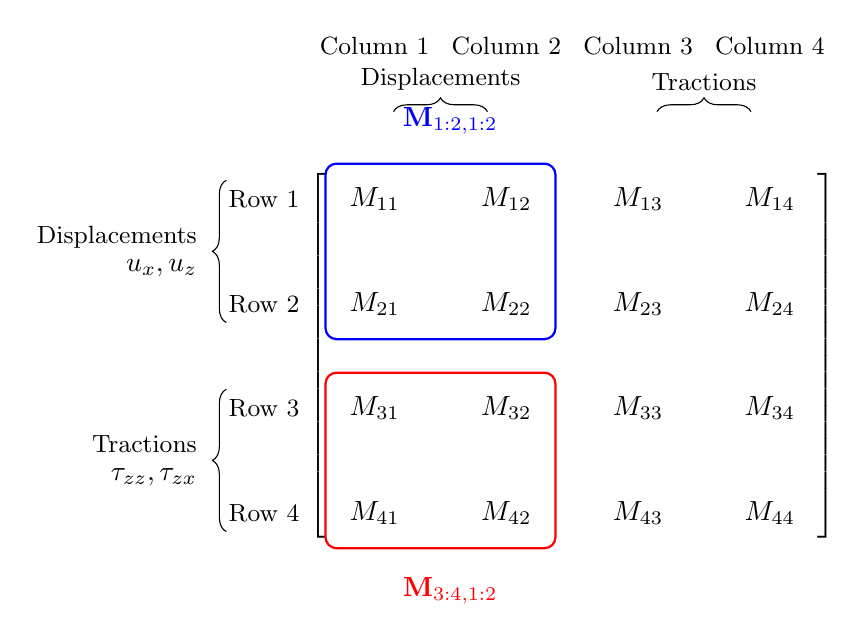
\begin{tikzpicture}[scale=1.2]

% Matrix
\matrix (M) [matrix of math nodes,
             left delimiter={[},
             right delimiter={]},
             row sep=0.8cm,
             column sep=0.8cm,
             ampersand replacement=\&] {
M_{11} \& M_{12} \& M_{13} \& M_{14} \\
M_{21} \& M_{22} \& M_{23} \& M_{24} \\
M_{31} \& M_{32} \& M_{33} \& M_{34} \\
M_{41} \& M_{42} \& M_{43} \& M_{44} \\
};

% Highlight blocks
\draw[blue, thick, rounded corners]
  ($(M-1-1.north west)+(-0.15,0.15)$)
  rectangle
  ($(M-2-2.south east)+(0.15,-0.15)$);

\node[blue] at ($(M-1-1.north)+(0.8,0.6)$)
  {$\mathbf{M}_{1:2,1:2}$};

\draw[red, thick, rounded corners]
  ($(M-3-1.north west)+(-0.15,0.15)$)
  rectangle
  ($(M-4-2.south east)+(0.15,-0.15)$);

\node[red] at ($(M-4-1.south)+(0.8,-0.6)$)
  {$\mathbf{M}_{3:4,1:2}$};

% Column labels
\node at ($(M-1-1.north)+(0,1.4)$) {\small Column 1};
\node at ($(M-1-2.north)+(0,1.4)$) {\small Column 2};
\node at ($(M-1-3.north)+(0,1.4)$) {\small Column 3};
\node at ($(M-1-4.north)+(0,1.4)$) {\small Column 4};

% Row labels
\node at ($(M-1-1.west)+(-0.8,0)$) {\small Row 1};
\node at ($(M-2-1.west)+(-0.8,0)$) {\small Row 2};
\node at ($(M-3-1.west)+(-0.8,0)$) {\small Row 3};
\node at ($(M-4-1.west)+(-0.8,0)$) {\small Row 4};

% Left braces (physical meaning)
\draw[decorate, decoration={brace, mirror, amplitude=5pt}]
  ($(M-1-1.west)+(-1.2,0.2)$) --
  ($(M-2-1.west)+(-1.2,-0.2)$)
  node[midway, left=0.25cm, align=right]
  {\small Displacements\\[-2pt]$\small u_x, u_z$};

\draw[decorate, decoration={brace, mirror, amplitude=5pt}]
  ($(M-3-1.west)+(-1.2,0.2)$) --
  ($(M-4-1.west)+(-1.2,-0.2)$)
  node[midway, left=0.25cm, align=right]
  {\small Tractions\\[-2pt]$\small \tau_{zz}, \tau_{zx}$};

% Top braces
\draw[decorate, decoration={brace, amplitude=5pt}]
  ($(M-1-1.north)+(0.2,0.7)$) --
  ($(M-1-2.north)+(-0.2,0.7)$)
  node[midway, above=0.15cm] {\small Displacements};

\draw[decorate, decoration={brace, amplitude=5pt}]
  ($(M-1-3.north)+(0.2,0.7)$) --
  ($(M-1-4.north)+(-0.2,0.7)$)
  node[midway, above=0.15cm] {\small Tractions};

\end{tikzpicture}
\end{center}

\section{The Halfspace Traction Matrix $\mathbf{T}_H$}

The halfspace traction operator is a $2 \times 2$ matrix:
\begin{equation}
\mathbf{T}_H = \begin{bmatrix}
T_{11} & T_{12} \\
T_{21} & T_{22}
\end{bmatrix}_{2 \times 2}
\end{equation}

where:
\begin{align}
T_{11} &= \lambda(-k^2 - q_P^2) + 2\mu q_P^2 \\
T_{12} &= 2i\mu k q_S \\
T_{21} &= -2i\mu k q_P \\
T_{22} &= -\mu(q_S^2 + k^2)
\end{align}

\textbf{Physical meaning:} $\mathbf{T}_H$ relates halfspace displacements to halfspace tractions for downgoing (decaying) waves only:
\begin{equation}
\begin{bmatrix}
\tau_{zz} \\
\tau_{zx}
\end{bmatrix}_{\text{halfspace}}
= \mathbf{T}_H
\begin{bmatrix}
u_x \\
u_z
\end{bmatrix}_{\text{halfspace}}
\end{equation}

\section{Putting It All Together}

\subsection{Step-by-Step Assembly}

\textbf{Step 1:} Surface displacements propagate to halfspace displacements
\begin{equation}
\begin{bmatrix}
u_x \\
u_z
\end{bmatrix}_{\text{halfspace}}
= \mathbf{M}_{1:2, 1:2}
\begin{bmatrix}
u_x \\
u_z
\end{bmatrix}_{\text{surface}}
\end{equation}

\textbf{Step 2:} Halfspace displacements create halfspace tractions
\begin{equation}
\begin{bmatrix}
\tau_{zz} \\
\tau_{zx}
\end{bmatrix}_{\text{halfspace}}
= \mathbf{T}_H
\begin{bmatrix}
u_x \\
u_z
\end{bmatrix}_{\text{halfspace}}
= \mathbf{T}_H \mathbf{M}_{1:2, 1:2}
\begin{bmatrix}
u_x \\
u_z
\end{bmatrix}_{\text{surface}}
\end{equation}

\textbf{Step 3:} Direct relationship between surface displacements and halfspace tractions
\begin{equation}
\begin{bmatrix}
\tau_{zz} \\
\tau_{zx}
\end{bmatrix}_{\text{halfspace}}
= \mathbf{M}_{3:4, 1:2}
\begin{bmatrix}
u_x \\
u_z
\end{bmatrix}_{\text{surface}}
\end{equation}

\textbf{Step 4:} For consistency, these two expressions must match:
\begin{equation}
\mathbf{M}_{3:4, 1:2}
\begin{bmatrix}
u_x \\
u_z
\end{bmatrix}_{\text{surface}}
+ \mathbf{T}_H \mathbf{M}_{1:2, 1:2}
\begin{bmatrix}
u_x \\
u_z
\end{bmatrix}_{\text{surface}}
= 0
\end{equation}

This must hold for arbitrary surface displacements, so:
\begin{equation}
\boxed{\mathbf{M}_{3:4, 1:2} + \mathbf{T}_H \mathbf{M}_{1:2, 1:2} = \mathbf{0}}
\end{equation}

\subsection{The Secular Equation}

For Rayleigh waves (free surface: $\tau_{zz} = \tau_{zx} = 0$ at $z=0$), non-trivial solutions exist only when:
\begin{equation}
\boxed{\det\left[\mathbf{M}_{3:4, 1:2} + \mathbf{T}_H \mathbf{M}_{1:2, 1:2}\right] = 0}
\end{equation}

This is the \textbf{Rayleigh wave secular equation}.

\section{Numerical Example}

Let's work through a concrete example with actual numbers.

\subsection{Sample Matrix Values}

Suppose at some $(c, \omega)$ we computed:
\begin{equation}
\mathbf{M} = \begin{bmatrix}
0.5 + 0.2i & 0.3 - 0.1i & 0.1 & 0.05 \\
-0.4 + 0.3i & 0.6 + 0.1i & -0.2 & 0.15 \\
200 + 50i & 150 - 30i & 100 & 80 \\
-180 + 40i & 190 + 20i & -120 & 110
\end{bmatrix}
\end{equation}

and:
\begin{equation}
\mathbf{T}_H = \begin{bmatrix}
300 + 100i & 50 - 20i \\
-60 + 30i & -250 - 80i
\end{bmatrix}
\end{equation}

\subsection{Extract Sub-Matrices}

\textbf{Extract $\mathbf{M}_{1:2, 1:2}$:}
\begin{equation}
\mathbf{M}_{1:2, 1:2} = \begin{bmatrix}
0.5 + 0.2i & 0.3 - 0.1i \\
-0.4 + 0.3i & 0.6 + 0.1i
\end{bmatrix}
\end{equation}

\textbf{Extract $\mathbf{M}_{3:4, 1:2}$:}
\begin{equation}
\mathbf{M}_{3:4, 1:2} = \begin{bmatrix}
200 + 50i & 150 - 30i \\
-180 + 40i & 190 + 20i
\end{bmatrix}
\end{equation}

\subsection{Compute the Product}

\begin{equation}
\mathbf{T}_H \mathbf{M}_{1:2, 1:2} = \begin{bmatrix}
300 + 100i & 50 - 20i \\
-60 + 30i & -250 - 80i
\end{bmatrix}
\begin{bmatrix}
0.5 + 0.2i & 0.3 - 0.1i \\
-0.4 + 0.3i & 0.6 + 0.1i
\end{bmatrix}
\end{equation}

(Work through matrix multiplication...)

\subsection{Form the Secular Matrix}

\begin{equation}
\mathbf{A} = \mathbf{M}_{3:4, 1:2} + \mathbf{T}_H \mathbf{M}_{1:2, 1:2}
\end{equation}

\subsection{Check the Determinant}

\begin{equation}
f(c, \omega) = \det(\mathbf{A})
\end{equation}

\begin{itemize}
    \item If $f(c, \omega) \approx 0$: We found a Rayleigh mode!
    \item If $f(c, \omega) \neq 0$: Keep searching for roots
\end{itemize}

\section{Python Code Correspondence}

In the actual Python implementation:

\begin{verbatim}
# Python uses 0-based indexing
# Mathematical M[3:4, 1:2] becomes M[2:4, 0:2]

# Extract sub-matrices
M_top = M[0:2, 0:2]      # M[1:2, 1:2] in math notation
M_bot = M[2:4, 0:2]      # M[3:4, 1:2] in math notation

# Form secular matrix
A = M_bot + TH @ M_top

# Compute determinant
det_A = np.linalg.det(A)
return np.real(det_A)
\end{verbatim}

\section{Summary}

\begin{itemize}
    \item \textbf{$\mathbf{M}_{1:2, 1:2}$:} Top-left $2\times2$ block (rows 1-2, columns 1-2)\\
    Connects: surface displacements $\rightarrow$ halfspace displacements
    
    \item \textbf{$\mathbf{M}_{3:4, 1:2}$:} Bottom-left $2\times2$ block (rows 3-4, columns 1-2)\\
    Connects: surface displacements $\rightarrow$ halfspace tractions
    
    \item \textbf{$\mathbf{T}_H$:} $2\times2$ halfspace operator\\
    Connects: halfspace displacements $\rightarrow$ halfspace tractions
    
    \item \textbf{Secular equation:} $\det[\mathbf{M}_{3:4, 1:2} + \mathbf{T}_H \mathbf{M}_{1:2, 1:2}] = 0$\\
    Enforces: free surface + radiation condition simultaneously
\end{itemize}

\end{document}



















